% Options for packages loaded elsewhere
\PassOptionsToPackage{unicode}{hyperref}
\PassOptionsToPackage{hyphens}{url}
%
\documentclass[
  12pt,
]{article}
\title{Impacts of Dam Removal on the Shenandoah River}
\usepackage{etoolbox}
\makeatletter
\providecommand{\subtitle}[1]{% add subtitle to \maketitle
  \apptocmd{\@title}{\par {\large #1 \par}}{}{}
}
\makeatother
\subtitle{\url{https://github.com/lydiecos/WDA-Dam-Removal}}
\author{Lydie Costes}
\date{}

\usepackage{amsmath,amssymb}
\usepackage{lmodern}
\usepackage{iftex}
\ifPDFTeX
  \usepackage[T1]{fontenc}
  \usepackage[utf8]{inputenc}
  \usepackage{textcomp} % provide euro and other symbols
\else % if luatex or xetex
  \usepackage{unicode-math}
  \defaultfontfeatures{Scale=MatchLowercase}
  \defaultfontfeatures[\rmfamily]{Ligatures=TeX,Scale=1}
  \setmainfont[]{Times New Roman}
\fi
% Use upquote if available, for straight quotes in verbatim environments
\IfFileExists{upquote.sty}{\usepackage{upquote}}{}
\IfFileExists{microtype.sty}{% use microtype if available
  \usepackage[]{microtype}
  \UseMicrotypeSet[protrusion]{basicmath} % disable protrusion for tt fonts
}{}
\makeatletter
\@ifundefined{KOMAClassName}{% if non-KOMA class
  \IfFileExists{parskip.sty}{%
    \usepackage{parskip}
  }{% else
    \setlength{\parindent}{0pt}
    \setlength{\parskip}{6pt plus 2pt minus 1pt}}
}{% if KOMA class
  \KOMAoptions{parskip=half}}
\makeatother
\usepackage{xcolor}
\IfFileExists{xurl.sty}{\usepackage{xurl}}{} % add URL line breaks if available
\IfFileExists{bookmark.sty}{\usepackage{bookmark}}{\usepackage{hyperref}}
\hypersetup{
  pdftitle={Impacts of Dam Removal on the Shenandoah River},
  pdfauthor={Lydie Costes},
  hidelinks,
  pdfcreator={LaTeX via pandoc}}
\urlstyle{same} % disable monospaced font for URLs
\usepackage[margin=2.54cm]{geometry}
\usepackage{longtable,booktabs,array}
\usepackage{calc} % for calculating minipage widths
% Correct order of tables after \paragraph or \subparagraph
\usepackage{etoolbox}
\makeatletter
\patchcmd\longtable{\par}{\if@noskipsec\mbox{}\fi\par}{}{}
\makeatother
% Allow footnotes in longtable head/foot
\IfFileExists{footnotehyper.sty}{\usepackage{footnotehyper}}{\usepackage{footnote}}
\makesavenoteenv{longtable}
\usepackage{graphicx}
\makeatletter
\def\maxwidth{\ifdim\Gin@nat@width>\linewidth\linewidth\else\Gin@nat@width\fi}
\def\maxheight{\ifdim\Gin@nat@height>\textheight\textheight\else\Gin@nat@height\fi}
\makeatother
% Scale images if necessary, so that they will not overflow the page
% margins by default, and it is still possible to overwrite the defaults
% using explicit options in \includegraphics[width, height, ...]{}
\setkeys{Gin}{width=\maxwidth,height=\maxheight,keepaspectratio}
% Set default figure placement to htbp
\makeatletter
\def\fps@figure{htbp}
\makeatother
\setlength{\emergencystretch}{3em} % prevent overfull lines
\providecommand{\tightlist}{%
  \setlength{\itemsep}{0pt}\setlength{\parskip}{0pt}}
\setcounter{secnumdepth}{5}
\ifLuaTeX
  \usepackage{selnolig}  % disable illegal ligatures
\fi

\begin{document}
\maketitle

\newpage

\hypertarget{rationale-and-research-questions}{%
\section{Rationale and Research
Questions}\label{rationale-and-research-questions}}

Over the past century, perceptions of dams have gradually changed, as
understanding of their serious ecological issues has increased and as
existing dams have aged, creating safety concerns and the need for
expensive repairs. Dams block the passage of fish and other aquatic
species, seriously disrupting life cycles for some species. They also
impact water quality and alter natural flow. Increasingly, dam removal
is pursued as an option to deal with aging dams and restore rivers.

In this study, we seek to understand how dam removal has impacted the
physical and chemical processes of one river, the Neuse River in North
Carolina. From 2004-2005, three dams were removed from the Southern Fork
of the Shenandoah River (see map below). The gage we are using for these
analyses is downstream from these dams and should thus reflect some of
the changes in flow and water quality that occurred after these
removals.

Below: The red X marks the spot of the McGaheysville Dam, which were
removed along with the Knightly Dam and Rockland Dam upstream in
2004-2005. All three dams were located along the south fork of the
Shenandoah River, which feeds into the Potomac.

\begin{figure}
\centering
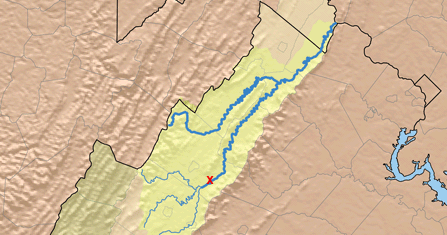
\includegraphics{../Figures-and-Maps/mcgaheysvilledam.png}
\caption{map of Neuse River}
\end{figure}

We are interested in both changes in physical process and changes in
chemical processes, which can vary widely according to the specific
river, its history, and the dam removal process (Foley et al 2017). Dams
allow for moderation of flow, often eliminating extreme flooding events.
Therefore, dam removal in combination with increasing extreme weather
events due to climate change could lead to more extreme and more
frequent high flow events. On the other hand, natural river systems and
riparian areas can be more resilient to flood events than artificially
constructed channels, so true restoration could help mitigate high flow
events to some extent.

Changes in water quality are also an area of interest. Large amounts of
sediment and minerals built up behind the dam may release quickly after
removal, especially if the removal was sudden rather than gradual (Foley
et al 2017). Over longer time, water quality is expected to improve
because of restored ecological processes.

\begin{enumerate}
\def\labelenumi{\arabic{enumi}.}
\item
  Question 1: Have discharge levels become more extreme since dam
  removal?
\item
  Question 2: Has there been a change in release of sediment and
  nutrients since the dam removal?
\end{enumerate}

\newpage

\hypertarget{dataset-information}{%
\section{Dataset Information}\label{dataset-information}}

The dataset consists of discharge and water quality data from stream
gage \#01631000, which is located on the South Fork of the Shenandoah
River downstream from the three dam removal sites. These data were
obtained from USGS StreamStats: \url{https://streamstats.usgs.gov/ss/}.

The dataset includes 183 parameters, but these parameters vary widely in
terms of how many datapoints were collected. To choose water quality
variables, I made a list of the top ten water quality parameters
according to the number of observations, and then selected three that I
thought would be particularly interesting and informative in light of
dam removal. These three were: suspended sediments, nitrogen, and
phosphate. Temperature is also included in the exploratory analyses. All
of these variables could be expected to change after dam removal.

\hypertarget{data-wrangling}{%
\subsection{Data Wrangling}\label{data-wrangling}}

The data were downloaded as two separate datasets: discharge
(`ShenaFlow') and water quality (`ShenaWQ'). Column names were changed
from defaults to be more comprehensible. Month and Year columns were
added to each dataset.

The discharge dataset was summarized into two dataframes, one by month
and the other by year. In both cases, discharge minimum, mean, and
maximum were calculated according to the summary unit.

The water quality dataset was transformed into a wider dataset with the
four parameters of interest divided into separate columns, instead of
being compiled in two columns by characteristic and value. The resulting
dataframe was also summarized by month, with minimum, mean, and maximum
calculated for each of the four parameters.

\begin{longtable}[]{@{}lrrrrrrrr@{}}
\toprule
& vars & n & mean & sd & min & max & range & se \\
\midrule
\endhead
Discharge & 1 & 33451 & 1602.889 & 2563.372 & 103 & 114000 & 113897 &
14.01545 \\
\bottomrule
\end{longtable}

\begin{longtable}[]{@{}lrrrrrrrr@{}}
\toprule
& vars & n & mean & sd & min & max & range & se \\
\midrule
\endhead
Nitrogen\_mg.L & 1 & 589 & 0.9908829 & 0.4492672 & 0.01 & 2.69 & 2.68 &
0.0185117 \\
Temp\_C & 2 & 767 & 14.2938722 & 8.2711759 & -0.10 & 30.50 & 30.60 &
0.2986549 \\
Phosphate\_mg.L & 3 & 582 & 0.2240997 & 0.2547145 & 0.00 & 1.93 & 1.93 &
0.0105583 \\
Sediments\_mg.L & 4 & 471 & 54.7594055 & 150.6138832 & 0.00 & 2020.00 &
2020.00 & 6.9399214 \\
\bottomrule
\end{longtable}

\newpage

\hypertarget{exploratory-analysis}{%
\section{Exploratory Analysis}\label{exploratory-analysis}}

Below are exploratory plots showing each parameter over time.

\begin{figure}
\centering
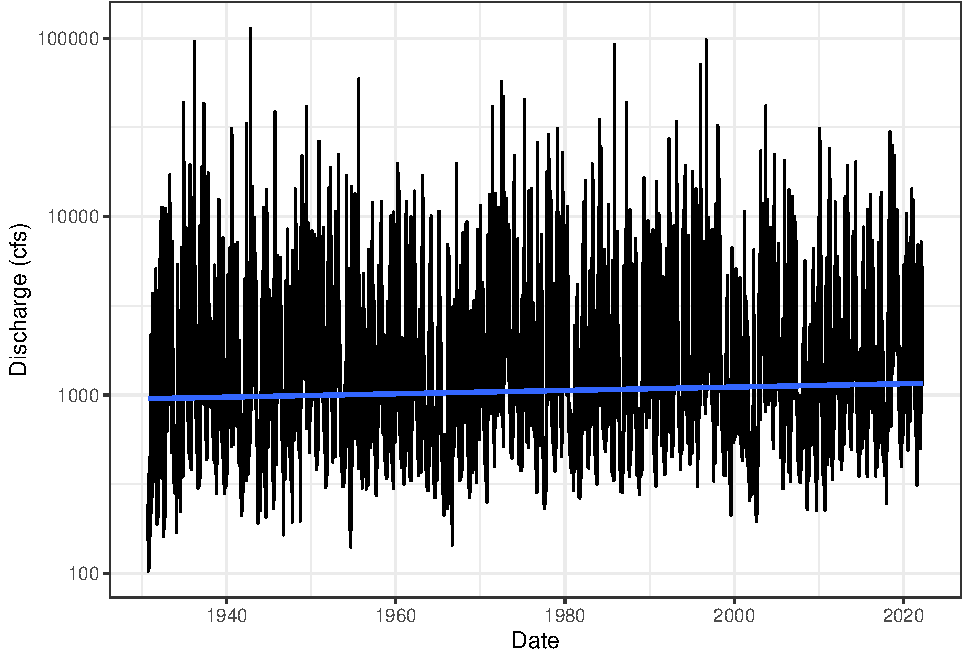
\includegraphics{Project_Template_files/figure-latex/exploration_plot1-1.pdf}
\caption{Discharge over time}
\end{figure}

\begin{figure}
\centering
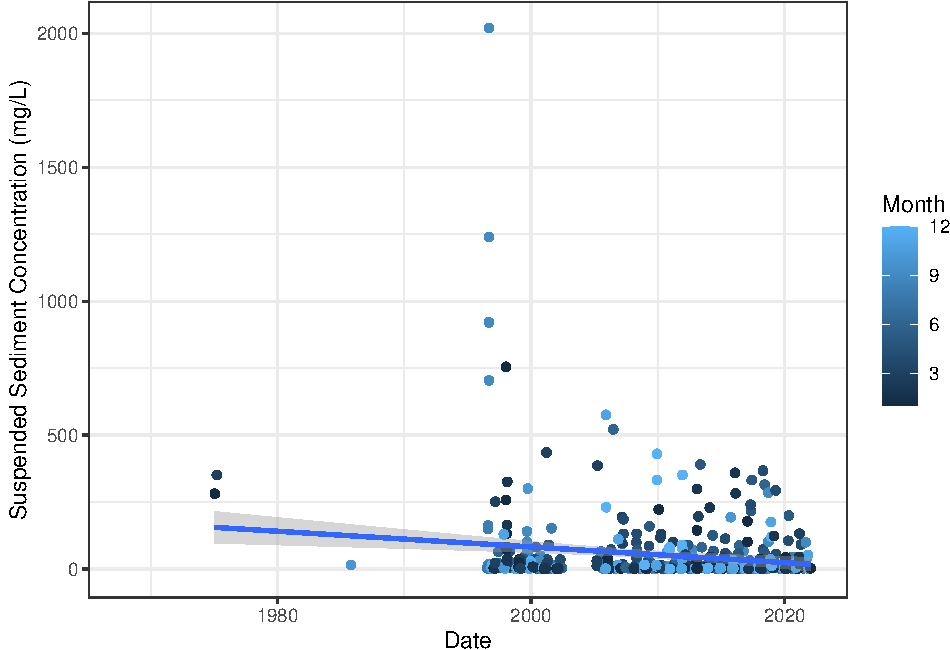
\includegraphics{Project_Template_files/figure-latex/exploration_plot2-1.pdf}
\caption{Sediment over time}
\end{figure}

\begin{figure}
\centering
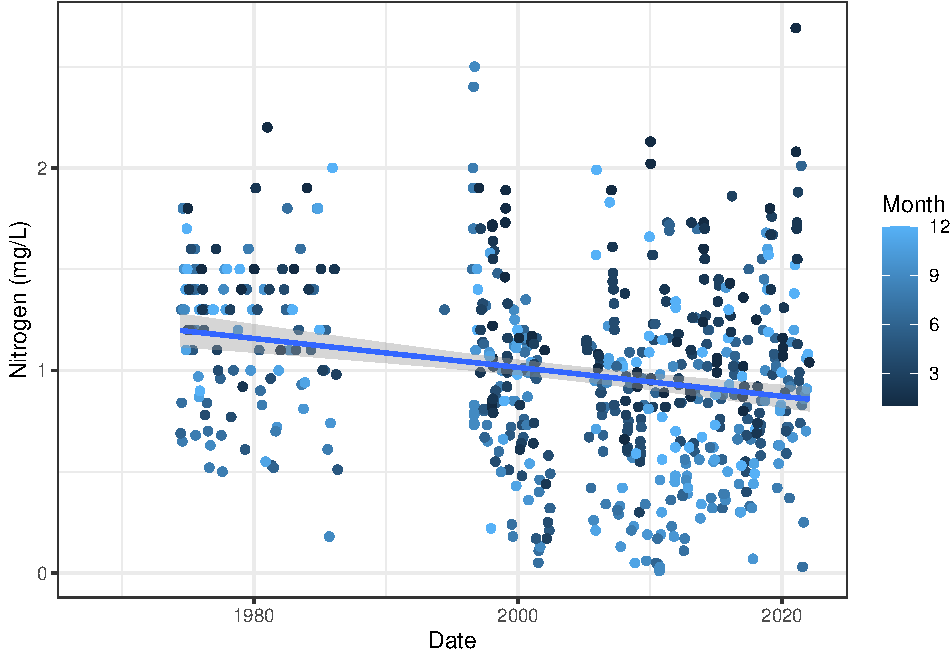
\includegraphics{Project_Template_files/figure-latex/exploration_plot3-1.pdf}
\caption{Nitrogen over time}
\end{figure}

\begin{figure}
\centering
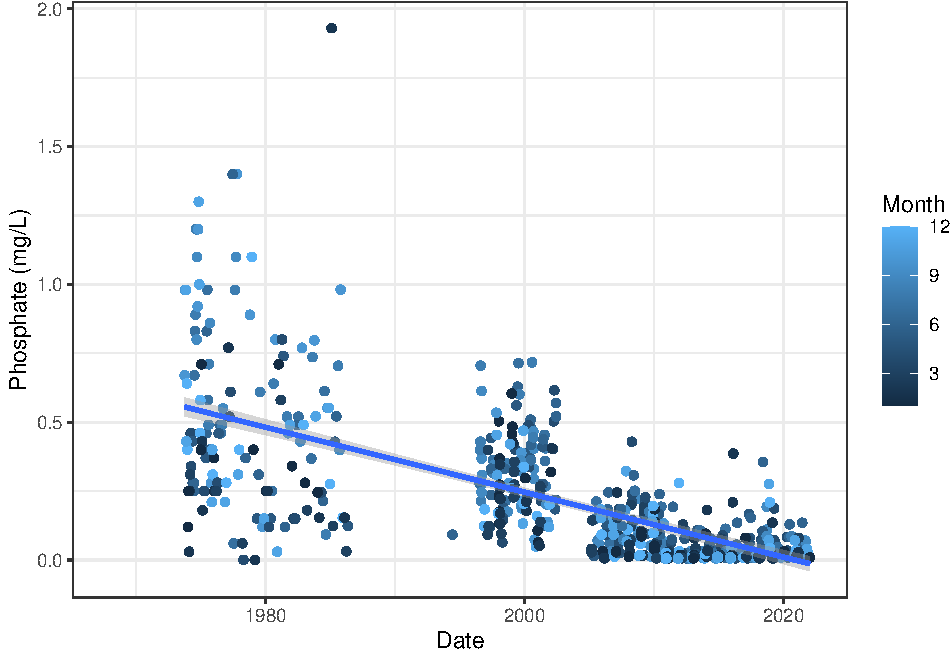
\includegraphics{Project_Template_files/figure-latex/exploration_plot4-1.pdf}
\caption{Phosphate over time}
\end{figure}

\begin{figure}
\centering
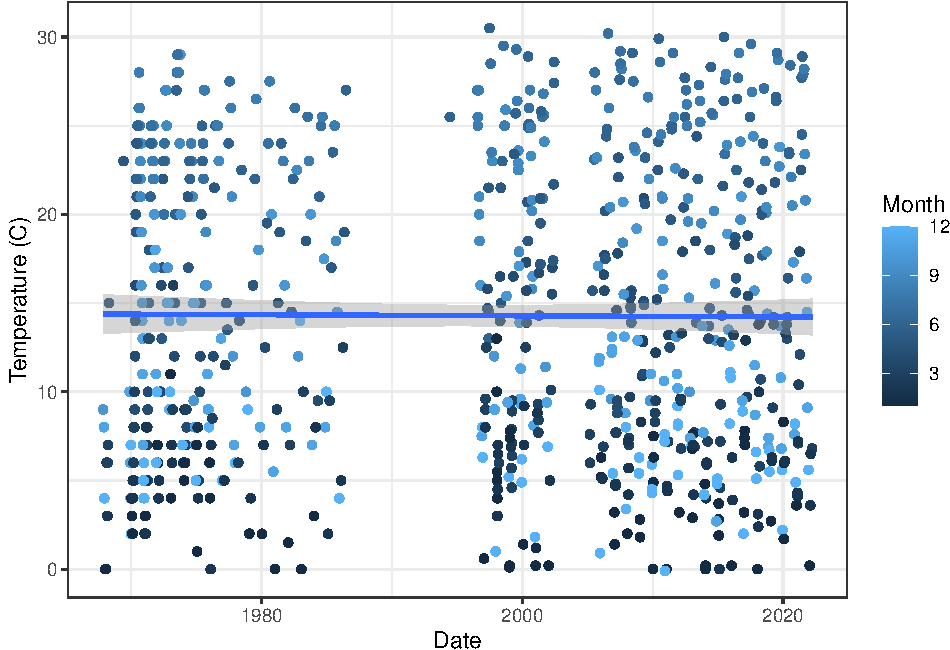
\includegraphics{Project_Template_files/figure-latex/exploration_plot5-1.pdf}
\caption{Temperature over time}
\end{figure}

\newpage

\hypertarget{analysis}{%
\section{Analysis}\label{analysis}}

\hypertarget{question-1-flow}{%
\subsection{Question 1: Flow}\label{question-1-flow}}

\begin{quote}
Question \#1: Have discharge extremes increased since the removal of the
dams? Has average discharge increased since dam removal?
\end{quote}

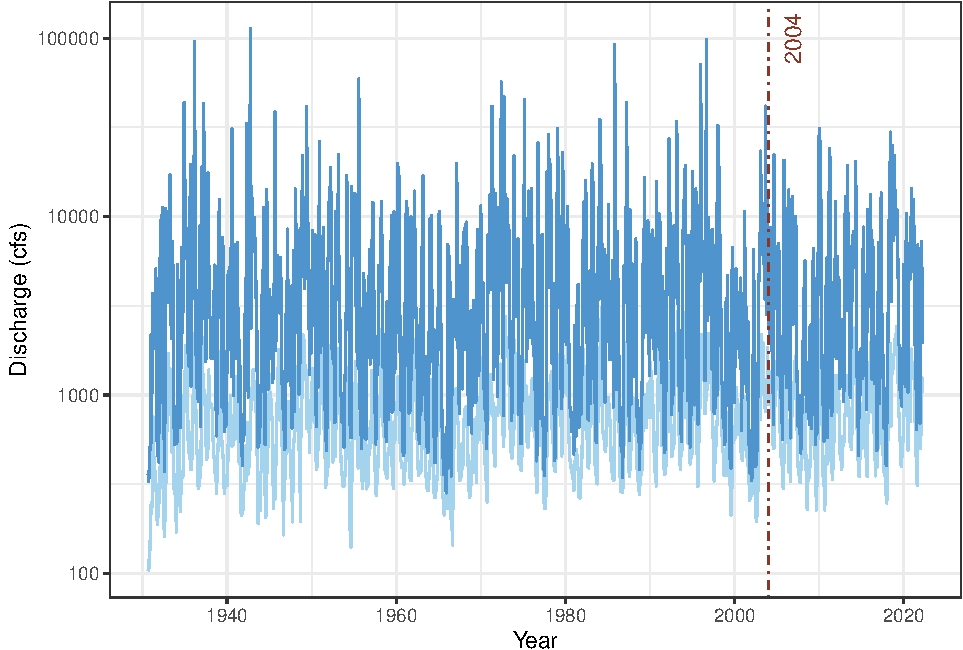
\includegraphics{Project_Template_files/figure-latex/Flow.analysis-1.pdf}
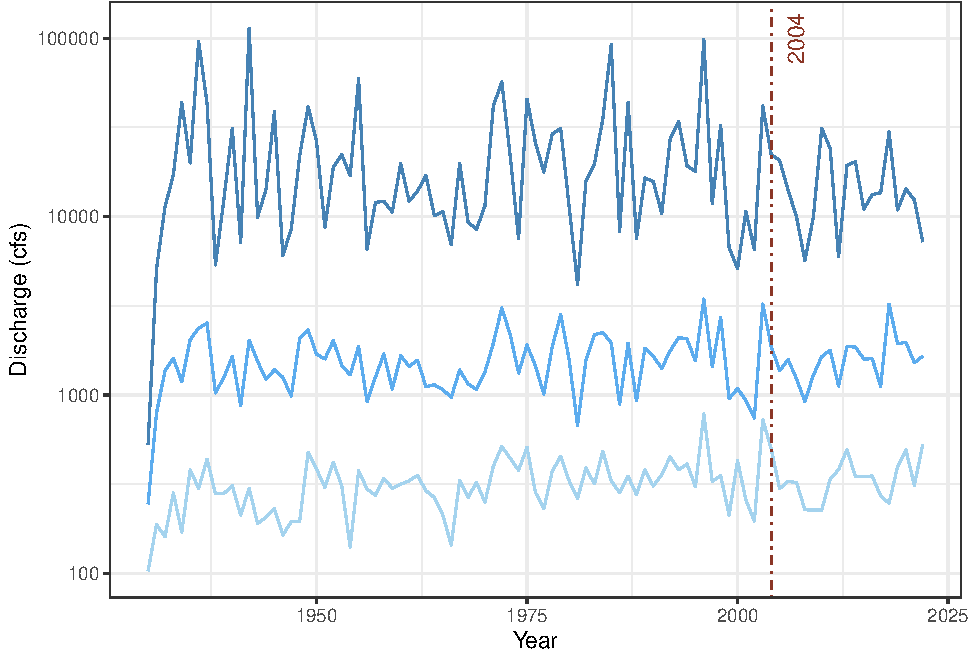
\includegraphics{Project_Template_files/figure-latex/Flow.analysis-2.pdf}

Maximum and minimum flows have not gotten more extreme since dam
removal.

\begin{longtable}[]{@{}llrrrrrrr@{}}
\caption{Summary Statistics for Discharge}\tabularnewline
\toprule
& Timeframe & n & mean & sd & min & max & range & se \\
\midrule
\endfirsthead
\toprule
& Timeframe & n & mean & sd & min & max & range & se \\
\midrule
\endhead
X1 & Before & 26764 & 1594.155 & 2687.319 & 103 & 114000 & 113897 &
16.42645 \\
X11 & After & 5956 & 1640.279 & 2009.455 & 226 & 31300 & 31074 &
26.03760 \\
\bottomrule
\end{longtable}

Average flow appears to be higher since dam removal. Verify with a
t-test:

\begin{verbatim}
## 
##  Welch Two Sample t-test
## 
## data:  ShenaFlow.before$Discharge and ShenaFlow.after$Discharge
## t = -1.4982, df = 11242, p-value = 0.1341
## alternative hypothesis: true difference in means is not equal to 0
## 95 percent confidence interval:
##  -106.47011   14.22224
## sample estimates:
## mean of x mean of y 
##  1594.155  1640.279
\end{verbatim}

Flow levels have not been significantly different before versus after
the dam removal (p = 0.140, df = 11202).

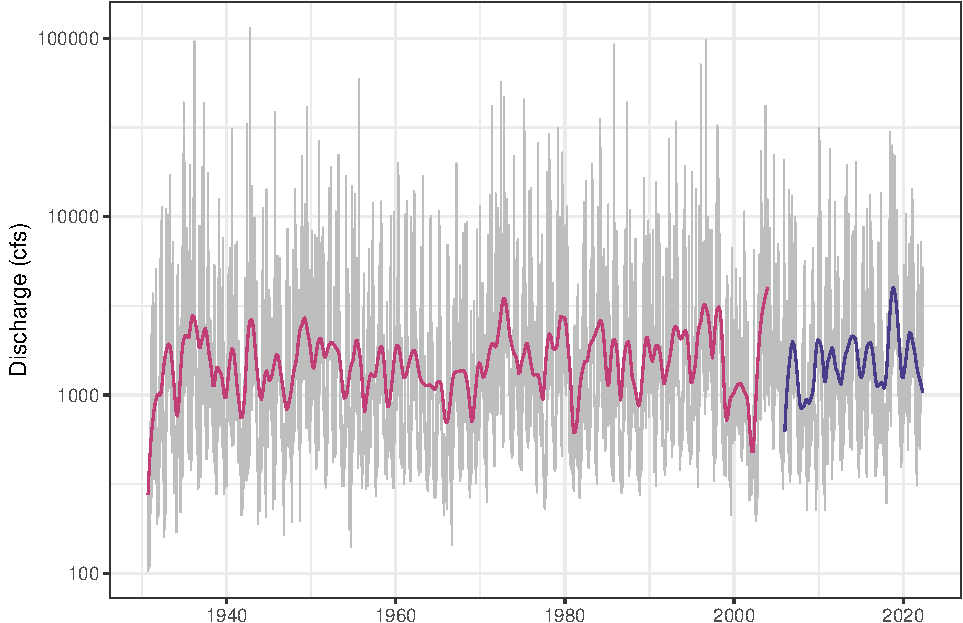
\includegraphics{Project_Template_files/figure-latex/flow_ts_graph-1.pdf}

\newpage

\hypertarget{question-2}{%
\subsection{Question 2}\label{question-2}}

\begin{quote}
Question \#2: Has there been a change in release of sediment and
nutrients since the dam removal?
\end{quote}

\hypertarget{sediment}{%
\subsubsection{Sediment}\label{sediment}}

\begin{quote}
Have sediment levels changed since dam removal?
\end{quote}

View summary statistics comparing sediment levels before versus after
dam removal:

\begin{longtable}[]{@{}llrrrrrrr@{}}
\caption{Summary Statistics for Sediment}\tabularnewline
\toprule
& Timeframe & n & mean & sd & min & max & range & se \\
\midrule
\endfirsthead
\toprule
& Timeframe & n & mean & sd & min & max & range & se \\
\midrule
\endhead
Sediments\_mg.L & Before & 137 & 83.15474 & 242.94443 & 0.3 & 2020 &
2019.7 & 20.756144 \\
Sediments\_mg.L1 & After & 321 & 40.64324 & 79.63389 & 0.0 & 521 & 521.0
& 4.444731 \\
\bottomrule
\end{longtable}

Test whether average sediment has been different before versus after dam
removal:

\begin{verbatim}
## 
##  Welch Two Sample t-test
## 
## data:  ShenaWQ.before$Sediments_mg.L and ShenaWQ.after$Sediments_mg.L
## t = 2.0027, df = 148.63, p-value = 0.04702
## alternative hypothesis: true difference in means is not equal to 0
## 95 percent confidence interval:
##   0.5663858 84.4566235
## sample estimates:
## mean of x mean of y 
##  83.15474  40.64324
\end{verbatim}

\newpage

\hypertarget{nitrogen}{%
\subsubsection{Nitrogen}\label{nitrogen}}

Have nitrogen levels changed since dam removal?

View summary statistics comparing nitrogen levels before versus after
dam removal:

\begin{longtable}[]{@{}llrrrrrrr@{}}
\caption{Summary Statistics for Nitrogen}\tabularnewline
\toprule
& Timeframe & n & mean & sd & min & max & range & se \\
\midrule
\endfirsthead
\toprule
& Timeframe & n & mean & sd & min & max & range & se \\
\midrule
\endhead
Nitrogen\_mg.L & Before & 254 & 1.0861811 & 0.4326022 & 0.05 & 2.50 &
2.45 & 0.0271439 \\
Nitrogen\_mg.L1 & After & 323 & 0.9178328 & 0.4466726 & 0.01 & 2.69 &
2.68 & 0.0248535 \\
\bottomrule
\end{longtable}

Visualize yearly minimum, mean, and maximum nitrogen levels:

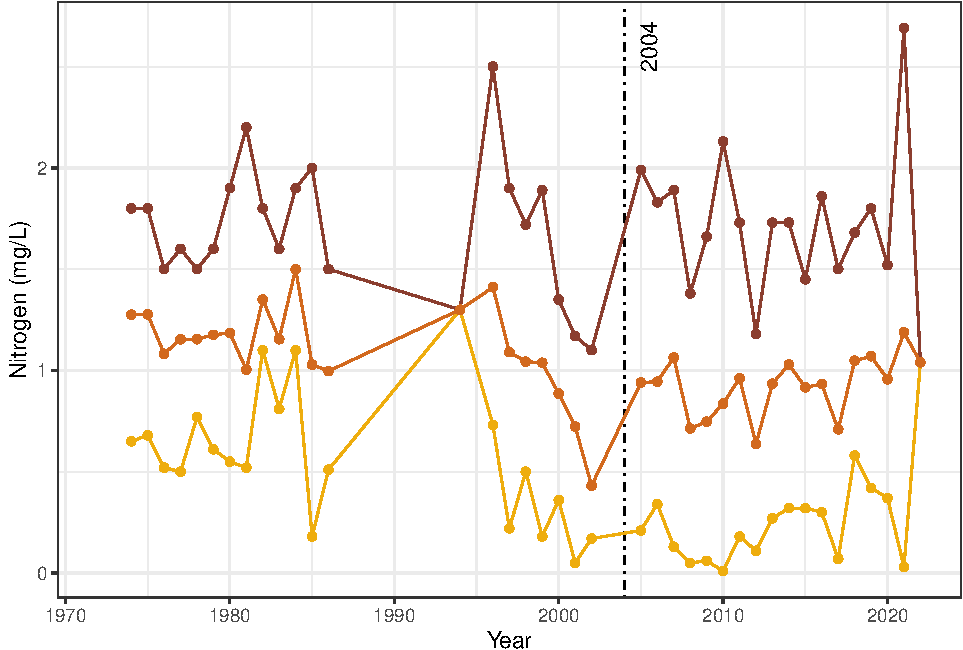
\includegraphics{Project_Template_files/figure-latex/Nitrogen_Analysis3-1.pdf}

Check whether average nitrogen levels have changed since dam removal:

\begin{verbatim}
## 
##  Welch Two Sample t-test
## 
## data:  ShenaWQ.before$Nitrogen_mg.L and ShenaWQ.after$Nitrogen_mg.L
## t = 4.5743, df = 550.84, p-value = 0.000005908
## alternative hypothesis: true difference in means is not equal to 0
## 95 percent confidence interval:
##  0.09605617 0.24064040
## sample estimates:
## mean of x mean of y 
## 1.0861811 0.9178328
\end{verbatim}

Yes, nitrogen levels since dam removal (M = 0.92, SD = 0.45) have been
significantly lower (t(550.8) = 4.56, p \textless{} 0.001) compared with
nitrogen levels before dam removal (M = 1.09, sd = 0.43).

\newpage

\hypertarget{phosphate}{%
\subsubsection{Phosphate}\label{phosphate}}

View summary statistics comparing sediment levels before versus after
dam removal:

\begin{longtable}[]{@{}llrrrrrrr@{}}
\caption{Summary Statistics for Phosphate}\tabularnewline
\toprule
& Timeframe & n & mean & sd & min & max & range & se \\
\midrule
\endfirsthead
\toprule
& Timeframe & n & mean & sd & min & max & range & se \\
\midrule
\endhead
Phosphate\_mg.L & Before & 272 & 0.3984853 & 0.2743858 & 0.000 & 1.930 &
1.930 & 0.0166371 \\
Phosphate\_mg.L1 & After & 297 & 0.0692997 & 0.0755835 & 0.006 & 0.429 &
0.423 & 0.0043858 \\
\bottomrule
\end{longtable}

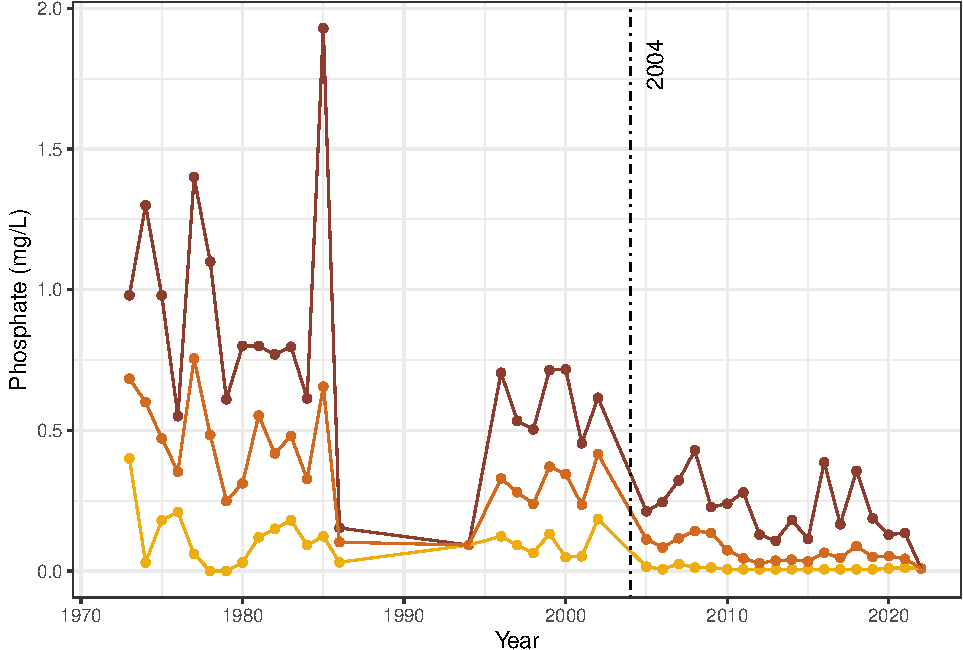
\includegraphics{Project_Template_files/figure-latex/Phosphate_Analysis3-1.pdf}

Test whether phosphate levels were different before versus after dam
removal:

\begin{verbatim}
## 
##  Welch Two Sample t-test
## 
## data:  ShenaWQ.before$Phosphate_mg.L and ShenaWQ.after$Phosphate_mg.L
## t = 19.133, df = 308.61, p-value < 2.2e-16
## alternative hypothesis: true difference in means is not equal to 0
## 95 percent confidence interval:
##  0.2953308 0.3630405
## sample estimates:
##  mean of x  mean of y 
## 0.39848529 0.06929966
\end{verbatim}

Phosphate levels have been significantly lower (t(309.22) = 19.10, p
\textless{} 0.001) since dam removal (M = 0.07, SD = 0.08) compared with
during the dammed years (M = 0.40, SD = 0.27).

\newpage

\hypertarget{summary-and-conclusions}{%
\section{Summary and Conclusions}\label{summary-and-conclusions}}

\begin{itemize}
\item
  Flow:
\item
  Sediment:
\item
  Both Nitrogen and Phosphate levels were significantly lower after dam
  removal.
\end{itemize}

\newpage

\hypertarget{references}{%
\section{References}\label{references}}

\begin{itemize}
\tightlist
\item
  Foley, M. M., J. R. Bellmore, J. E. O'Connor, J. J. Duda, A. E. East,
  G. E. Grant, C. W. Anderson, J. A. Bountry, M. J. Collins, P. J.
  Connolly, L. S. Craig, J. E. Evans, S. L. Greene,F. J. Magilligan, C.
  S. Magirl, J. J. Major, G. R. Pess,T. J. Randle, P. B. Shafroth, C. E.
  Torgersen, D. Tullos, A. C. Wilcox. 2017. Dam removal: Listening in.
  Water Resources Research. 53(7):5229-5246.
  \url{https://doi-org.proxy.lib.duke.edu/10.1002/2017WR020457}
\end{itemize}

Map source:
\url{http://www.virginiaplaces.org/watersheds/fishpassage.html}

Sediment deposits alter downstream tidal communities
\url{https://journals.plos.org/plosone/article?id=10.1371/journal.pone.0187742\#references}

info: \url{https://dwr.virginia.gov/fishing/fish-passage/\#orange}

\end{document}
